% Options for packages loaded elsewhere
\PassOptionsToPackage{unicode}{hyperref}
\PassOptionsToPackage{hyphens}{url}
%
\documentclass[
]{article}
\usepackage{lmodern}
\usepackage{amssymb,amsmath}
\usepackage{ifxetex,ifluatex}
\ifnum 0\ifxetex 1\fi\ifluatex 1\fi=0 % if pdftex
  \usepackage[T1]{fontenc}
  \usepackage[utf8]{inputenc}
  \usepackage{textcomp} % provide euro and other symbols
\else % if luatex or xetex
  \usepackage{unicode-math}
  \defaultfontfeatures{Scale=MatchLowercase}
  \defaultfontfeatures[\rmfamily]{Ligatures=TeX,Scale=1}
\fi
% Use upquote if available, for straight quotes in verbatim environments
\IfFileExists{upquote.sty}{\usepackage{upquote}}{}
\IfFileExists{microtype.sty}{% use microtype if available
  \usepackage[]{microtype}
  \UseMicrotypeSet[protrusion]{basicmath} % disable protrusion for tt fonts
}{}
\makeatletter
\@ifundefined{KOMAClassName}{% if non-KOMA class
  \IfFileExists{parskip.sty}{%
    \usepackage{parskip}
  }{% else
    \setlength{\parindent}{0pt}
    \setlength{\parskip}{6pt plus 2pt minus 1pt}}
}{% if KOMA class
  \KOMAoptions{parskip=half}}
\makeatother
\usepackage{xcolor}
\IfFileExists{xurl.sty}{\usepackage{xurl}}{} % add URL line breaks if available
\IfFileExists{bookmark.sty}{\usepackage{bookmark}}{\usepackage{hyperref}}
\hypersetup{
  pdftitle={Maternal sexual empowerment and early sexual onset among female adolescents: Evidence from a prevalence study in Ecuador},
  pdfauthor={Alonso Quijano},
  hidelinks,
  pdfcreator={LaTeX via pandoc}}
\urlstyle{same} % disable monospaced font for URLs
\usepackage[margin=1in]{geometry}
\usepackage{graphicx}
\makeatletter
\def\maxwidth{\ifdim\Gin@nat@width>\linewidth\linewidth\else\Gin@nat@width\fi}
\def\maxheight{\ifdim\Gin@nat@height>\textheight\textheight\else\Gin@nat@height\fi}
\makeatother
% Scale images if necessary, so that they will not overflow the page
% margins by default, and it is still possible to overwrite the defaults
% using explicit options in \includegraphics[width, height, ...]{}
\setkeys{Gin}{width=\maxwidth,height=\maxheight,keepaspectratio}
% Set default figure placement to htbp
\makeatletter
\def\fps@figure{htbp}
\makeatother
\setlength{\emergencystretch}{3em} % prevent overfull lines
\providecommand{\tightlist}{%
  \setlength{\itemsep}{0pt}\setlength{\parskip}{0pt}}
\setcounter{secnumdepth}{-\maxdimen} % remove section numbering
\usepackage{dcolumn}
\usepackage{pdflscape}
\newcommand{\blandscape}{\begin{landscape}}
\newcommand{\elandscape}{\end{landscape}}
\usepackage{fancyhdr}
\usepackage{booktabs}
\usepackage{longtable}
\usepackage{array}
\usepackage{multirow}
\usepackage{wrapfig}
\usepackage{float}
\usepackage{colortbl}
\usepackage{pdflscape}
\usepackage{tabu}
\usepackage{threeparttable}
\usepackage{threeparttablex}
\usepackage[normalem]{ulem}
\usepackage{makecell}
\usepackage{xcolor}
\newlength{\cslhangindent}
\setlength{\cslhangindent}{1.5em}
\newenvironment{cslreferences}%
  {\setlength{\parindent}{0pt}%
  \everypar{\setlength{\hangindent}{\cslhangindent}}\ignorespaces}%
  {\par}

\title{Maternal sexual empowerment and early sexual onset among female
adolescents: Evidence from a prevalence study in Ecuador}
\author{Alonso Quijano}
\date{}

\begin{document}
\maketitle

\emph{This study uses data from the 2018 National Health and Nutrition
Survey of Ecuador (Ensanut) to examine whether maternal sexual
empowerment is predictive of early sexual onset among female
adolescents. We used mothers' ability to turn down sex and demand
contraception as a measure of sexual empowerment. We also considered
mothers' age at first intercourse and whether they had experienced early
childbearing. Several logistic regressions were employed to estimate the
predicting value and significance of the variables of interest. Even
after controlling for several sociodemographic and economic confounders,
having a mother who lacked sexual empowerment was predictive of early
sexual activity. However, mothers' age at first intercourse was included
in the model, sexual empowerment was no longer significant, suggesting
that maternal sexual empowerment was predictive of sexual debut through
mothers' age at first intercourse. This study contributes to the
literature of early sexual initiation by exploring new connections in
which sexual values and behaviors may be transmitted from mother to
daughter. More research is needed confirm the robustness of these
results and analyze other forms of maternal empowerment.}

\hypertarget{introduction}{%
\subsection{INTRODUCTION}\label{introduction}}

The age of puberty onset has decreased substantially over the past
decades (Bellis et al., 2006). Reasons exist to be concerned about this
fact as early sexual debut has been linked to several adverse outcomes.
Early sexual initiators have been found to be more prone to having
multiple sex partners, forcing partners to have sex, having frequent
sexual intercourse, and being engaged in teenage pregnancy (O'Donnell et
al., 2001). Studies performed on different populations have also shown
an association between early initiation of sexual intercourse and HIV
and other STDs risks (e.g.~Kaestle et al., 2005; Stöckl et al., 2013).
One major cause of the high prevalence of STDs and unwanted pregnancies
among young males and females is that those who engage in early sexual
activityare much less likely to use contraception (Finer and Philbin,
2013). Additionally, even for those who manage to avoid pregnancy at
first intercourse despite not using contraception, chances of
experiencing early childbearing remain high since those who fail to use
contraception at first sex are more likely to continue engaging in risky
sexual behavior in the future (Magnusson et al., 2012; St Lawrence and
Scott, 1996).(INEC, 2019). (Xie, 2015)

Many studies have tested the relationship between precocious sexual
initiation and household structure (e.g.~Ellis et al., 2003; Newcomer
and Udry, 1987) and parental involvement (e.g.~Romer et al., 1999;
Sieverding et al., 2005; Velez-Pastrana et al., 2005). However, few
studies have explored the intergenerational transmission of behavioral
patterns, such as how the timing of sexual debut may be replicated
across generations (e.g.~Johnson and Tyler, 2007). This paper aims to
examine the predicting ability of maternal behavioral variables,
including the mother's age at first intercourse, and other mechanisms in
which the mother's control of her sexual decisions can be passed on to
her daughter's own decision making. It is plausible to believe that
those mothers with low bargaining power may directly or indirectly
transmit their norms and beliefs to their daughters, who may as well
then become unable to exercise decision-making over their sexuality.
Parkes et al.~(2011) found that talking about sex and contraception with
children was negatively correlated with delayed sexual initiation,
suggesting that parents may be able to shape their children's skills for
negotiating sexual situations. The influence intra-household sexual
bargaining has on children has yet been explored in experimental
research. Therefore, this study opens up an opportunity to discuss more
in depth how sexual values may be inherited and how they can relate to
the sexual well-being of young women.

\hypertarget{methods}{%
\subsection{METHODS}\label{methods}}

\hypertarget{data-and-sample}{%
\subsection{Data and sample}\label{data-and-sample}}

We used data from the 2018 National Health and Nutrition Survey of
Ecuador (Ensanut), which is conducted every five years by the National
Statistics Institute of Ecuador. Its goal is to assess the health and
nutritional status of adults and children in Ecuador. In 2018, the
survey gathered data from 43,311 households, totaling a number of
168,747 subjects. Measures of anthropometric, nutrition, economic status
were collected for all the members of the household. Data about the
sexual health of women was gathered for all those between 12 and 49
years old. Information about risk factors (e.g.~smoking and drinking)
was collected for only one random subject (male or female) between 5 and
18.

To perform the analysis, we selected the data of girls who were 16 years
old at the time of the interview and their mothers. Because the we are
interested on how mother-related variables such as sexual empowerment
may relate to early sexual debut among young females, we filtered those
girls who were currently living with their mothers and their mothers'
partner (which in most cases was the father). As mentioned before,
information regarding sexuality was only gathered for women at age 49 or
younger. Therefore, we only considered those whose mother was under that
age threshold. Finally, as data about smoking and drinking are not
available for every subject, we decided to perform the analysis on two
samples: one larger sample that does not include these additional
confounders and a smaller one that includes them.

\hypertarget{measures}{%
\subsection{Measures}\label{measures}}

As in most studies that use secondary data, not all variables necessary
to understand the sexual activity of young females were available in
Ensanut. Nevertheless, we still were able to add several of the factors
that have been previously associated with early sexual debut.

The dependent variable for the analysis was \emph{early sexual
activity}. The 16-year-old girls who reported having had sexual
intercourse were coded as 1, whereas those who reported being virgin
were coded as 0. The 16-year-old cutoff has been used in previous
studies to demarcate early onset of sexual activity (e.g.~Ellis et al.,
2003; Paul et al., 2000).

Basic sociodemographic and economic measures included ethnicity (whether
the girl identified herself as an ethnic minority), geographic area
(urban or rural), whether the girl was attending school, and household
income in US dollars. We used income as a measure of poverty. However,
evidence favors the use of consumption as a more effective tool to
measure well-being in developing countries (Meyer and Sullivan, 2003).
Since consumption was not available in the survey, we added other
variables which may relate to the economic status of the household,
including access to internet and the number of household members. The
number of household members was the most predicting factor for
impoverishment used in the Poverty Probability Index (Schreiner, 2015).

Individual-level measures consisted of knowledge about sexuality and
risk behaviors. Sexuality knowledge was estimated through questions
about menstruation, pregnancy, and AIDs. Girls were asked whether they
knew what was happening to their body when they hay their first period,
whether a woman could become pregnant at first intercourse, and whether
HIV could spread through handshake. They were also asked whether they
had ever learned about sexual relations, and if so, from whom they had
learned about (school, family, and others). Risk factors included
whether the girl had ever drunk alcohol or smoked in the past.

Mother-related variables included the mother's sexual bargaining
ability, age at first intercourse, and whether she had a teenage birth.
Mothers were asked if they could say no to their sexual partners
whenever they did not want to have sexual intercourse. For those who
were not using any form of contraception but would prefer to use one,
they were asked whether they thought their partner would be willing to
use it or not. Mothers who were unable to turn down sex or demand their
partner to use contraception were classified as low sexual bargaining.
We also considered variables such as occupation and education.

\hypertarget{results}{%
\subsection{RESULTS}\label{results}}

After cleaning up the data, the sample contained answers from 828
16-year-old girls and their respective mothers. Among those, 16.4\% had
ever had sexual intercourse, while 83.6\% had not. Before performing the
primary analysis, differences in the prevalence of early sexual onset
and their relationship with the explanatory variables were assessed
using the chi-square and t-test. The primary analysis was based on a
series of logistic regression models examining the association between
early sexual activity among young females and the characteristics of
their mothers after adjustment for covariates.

Table 1 shows the percentage and mean levels of the explanatory
variables by each group. Mean differences of the categorical and
continuous variables were tested using the chi-square and t-test,
respectively. Across the two groups, girls who were sexually active were
more likely to belong to an ethnic minority (p \textless{} .001), live
in a rural area (p \textless{} .05), lack internet access (p \textless{}
.001), and miss school (p \textless{} .001). As for sexuality knowledge,
they tended to incorrectly answer the question about AIDs (p \textless{}
.05) and not know what was happening to their body when they had their
first period (p \textless{} .001). Sexually active girls were more
likely to learn about sexuality from family (p \textless{} .05) and
other sources (e.g., internet) (p \textless{} .001). In contrast,
non-sexually active girls were more prone to learning from school (p
\textless{} .001).

\newpage
\begin{landscape}
\begin{table}[!h]

\caption{\label{tab:unnamed-chunk-2}Percentage and mean levels of explanatory variables by group}
\centering
\resizebox{\linewidth}{!}{
\begin{threeparttable}
\begin{tabular}[t]{lrrrlrrlrrl}
\toprule
\multicolumn{2}{c}{ } & \multicolumn{9}{c}{Daughters' sexual outcomes} \\
\cmidrule(l{3pt}r{3pt}){3-11}
\multicolumn{2}{c}{ } & \multicolumn{3}{c}{Early sexual initiation} & \multicolumn{3}{c}{Teenage pregnancy} & \multicolumn{3}{c}{Contraception use at first intercourse} \\
\cmidrule(l{3pt}r{3pt}){3-5} \cmidrule(l{3pt}r{3pt}){6-8} \cmidrule(l{3pt}r{3pt}){9-11}
  & Total & \makecell[c]{Has ever had\\sexual intercourse} & \makecell[c]{Has not had\\sexual intercourse} & p value & \makecell[c]{Has ever been\\ pregnant} & \makecell[c]{Has not been\\pregnant} & p value & \makecell[c]{Used\\contraception} & \makecell[c]{Did not use\\contraception} & p value\\
\midrule
\addlinespace[2em]
\multicolumn{11}{l}{\textit{Explanatory variables}}\\
\hspace{1em}Mother lacks sexual empowerment & 0.10 & 0.14 & 0.09 & 0.102 & 0.13 & 0.10 & 0.463 & 0.12 & 0.15 & 0.782\\
\hspace{1em}Mother had a teenage birth & 0.52 & 0.68 & 0.48 & 0.000 *** & 0.70 & 0.50 & 0.003 *** & 0.64 & 0.70 & 0.581\\
\hspace{1em}Mother's age at first intercourse & 17.38 & 16.11 & 17.64 & 0.000 *** & 16.07 & 17.48 & 0.000 *** & 16.49 & 15.81 & 0.104\\
\addlinespace[2em]
\multicolumn{11}{l}{\textit{Mother-related variables}}\\
\hspace{1em}Mother has a job & 0.60 & 0.67 & 0.59 & 0.059  * & 0.65 & 0.60 & 0.465 & 0.67 & 0.69 & 0.977\\
\hspace{1em}Mother finished primary school & 0.97 & 0.93 & 0.98 & 0.008 *** & 0.91 & 0.97 & 0.018 ** & 0.99 & 0.88 & 0.026 **\\
\hspace{1em}Mother finished high school & 0.53 & 0.49 & 0.54 & 0.272 & 0.43 & 0.54 & 0.129 & 0.62 & 0.40 & 0.009 ***\\
\hspace{1em}Mother finished college & 0.15 & 0.10 & 0.16 & 0.082  * & 0.10 & 0.16 & 0.290 & 0.21 & 0.02 & 0.001 ***\\
\addlinespace[2em]
\multicolumn{11}{l}{\textit{Daughter-related variables}}\\
\hspace{1em}Misses school & 0.08 & 0.27 & 0.05 & 0.000 *** & 0.36 & 0.06 & 0.000 *** & 0.15 & 0.36 & 0.005 ***\\
\hspace{1em}Lacked knowledge about period & 0.20 & 0.28 & 0.19 & 0.009 *** & 0.32 & 0.20 & 0.023 ** & 0.19 & 0.37 & 0.020 **\\
\hspace{1em}Knows about sexuality from family & 0.11 & 0.14 & 0.11 & 0.314 & 0.13 & 0.11 & 0.718 & 0.19 & 0.08 & 0.070  *\\
\hspace{1em}Knows about sexuality from school & 0.80 & 0.75 & 0.80 & 0.167 & 0.75 & 0.80 & 0.451 & 0.74 & 0.78 & 0.694\\
\hspace{1em}Knows about sexuality from other sources & 0.03 & 0.06 & 0.03 & 0.053  * & 0.06 & 0.03 & 0.414 & 0.05 & 0.06 & 1.000\\
\addlinespace[2em]
\multicolumn{11}{l}{\textit{Household-related variables}}\\
\hspace{1em}Ethnic minority & 0.22 & 0.30 & 0.20 & 0.008 *** & 0.26 & 0.21 & 0.419 & 0.15 & 0.42 & 0.000 ***\\
\hspace{1em}Rural area & 0.40 & 0.43 & 0.40 & 0.586 & 0.38 & 0.41 & 0.731 & 0.26 & 0.55 & 0.000 ***\\
\hspace{1em}Internet access & 0.43 & 0.30 & 0.46 & 0.000 *** & 0.26 & 0.44 & 0.005 *** & 0.45 & 0.17 & 0.000 ***\\
\hspace{1em}Household members & 5.60 & 6.04 & 5.51 & 0.001 *** & 6.65 & 5.52 & 0.000 *** & 5.38 & 6.65 & 0.000 ***\\
\hspace{1em}Household income & 600.53 & 715.27 & 577.84 & 0.736 & 532.07 & 605.71 & 0.901 & 996.21 & 493.36 & 0.054  *\\
\bottomrule
\end{tabular}
\begin{tablenotes}[para]
\item \textit{Note: } 
\item p values for comparison of percentagges using chi-square. p values for comparison of means using t-test. Ns = 401–828. *p < .1; **p < .05; ***p < .01
\end{tablenotes}
\end{threeparttable}}
\end{table}
\end{landscape}
\newpage

Mother characteristics significantly differed across groups. Mothers of
early sexual initiators were less likely to have finished primary school
(p \textless{} .01) and more likely to have become a teenage parent (p
\textless{} .001). As expected, early sexual initiators were more likely
to have been reared by a mother who had herself had her first coitus at
a very young age. Figure 1 illustrates the cumulative histogram of age
at first coitus of the mothers. The figure clearly shows that mothers of
early sexual initiators had their first coitus at a younger age than
mothers of those who were not sexually active. The mean age at first
coitus for each group was 16.11 (SD = 2.48) and 17.76 (SD = 2.79),
respectively. The t-test showed that these differences were unlikely to
have been due to chance (p \textless{} .001).

\newpage
\begin{landscape}
\begin{table}[!h]

\caption{\label{tab:unnamed-chunk-3}}
\centering
\resizebox{\linewidth}{!}{
\begin{threeparttable}
\begin{tabular}[t]{lrrrlrrlr}
\toprule
\multicolumn{2}{c}{ } & \multicolumn{3}{c}{Maternal sexual empowerment} & \multicolumn{3}{c}{Mother had teenage birth} & \multicolumn{1}{c}{ } \\
\cmidrule(l{3pt}r{3pt}){3-5} \cmidrule(l{3pt}r{3pt}){6-8}
  & Total & \makecell[c]{Lacks sexual\\empowerment} & \makecell[c]{Is sexually\\empowered} & p value & \makecell[c]{Teenage\\birth} & \makecell[c]{No teenage\\birth} & p value & \makecell[c]{Mother's age\\at first\\ intercourse}\\
\midrule
\addlinespace[2em]
\multicolumn{9}{l}{\textit{Mother-related variables}}\\
\hspace{1em}Mother has a job & 0.60 & 0.50 & 0.61 & 0.038 ** & 0.62 & 0.59 & 0.351 & 17.36\\
\hspace{1em}Mother finished primary school & 0.97 & 0.98 & 0.97 & 0.743 & 0.97 & 0.96 & 0.586 & 17.42\\
\hspace{1em}Mother finished high school & 0.53 & 0.46 & 0.54 & 0.169 & 0.47 & 0.59 & 0.000 *** & 17.97\\
\hspace{1em}Mother finished college & 0.15 & 0.09 & 0.16 & 0.122 & 0.11 & 0.20 & 0.000 *** & 18.89\\
\addlinespace[2em]
\multicolumn{9}{l}{\textit{Daughter-related variables}}\\
\hspace{1em}Misses school & 0.08 & 0.08 & 0.08 & 1.000 & 0.09 & 0.07 & 0.323 & 15.97\\
\hspace{1em}Lacked knowledge about period & 0.20 & 0.21 & 0.20 & 1.000 & 0.22 & 0.19 & 0.162 & 16.93\\
\hspace{1em}Knows about sexuality from family & 0.11 & 0.08 & 0.11 & 0.478 & 0.14 & 0.08 & 0.009 *** & 17.20\\
\hspace{1em}Knows about sexuality from school & 0.80 & 0.82 & 0.79 & 0.581 & 0.77 & 0.82 & 0.101 & 17.45\\
\hspace{1em}Knows about sexuality from other sources & 0.03 & 0.04 & 0.03 & 0.872 & 0.04 & 0.02 & 0.113 & 16.69\\
\addlinespace[2em]
\multicolumn{9}{l}{\textit{Household-related variables}}\\
\hspace{1em}Ethnic minority & 0.22 & 0.31 & 0.20 & 0.021 ** & 0.22 & 0.21 & 0.918 & 16.88\\
\hspace{1em}Rural area & 0.40 & 0.46 & 0.40 & 0.298 & 0.40 & 0.41 & 0.921 & 17.04\\
\hspace{1em}Internet access & 0.43 & 0.38 & 0.44 & 0.308 & 0.40 & 0.46 & 0.043 ** & 18.02\\
\hspace{1em}Household members & 5.60 & 5.85 & 5.57 & 0.161 & 5.84 & 5.33 & 0.000 *** & NA\\
\hspace{1em}Household income & 600.53 & 842.21 & 574.32 & 0.599 & 682.82 & 512.88 & 0.575 & NA\\
\bottomrule
\end{tabular}
\begin{tablenotes}[para]
\item \textit{Note: } 
\item p values for comparison of percentagges using chi-square. p values for comparison of means using t-test. Ns = 401–828. *p < .1; **p < .05; ***p < .01
\end{tablenotes}
\end{threeparttable}}
\end{table}
\end{landscape}
\newpage

\begin{figure}

{\centering 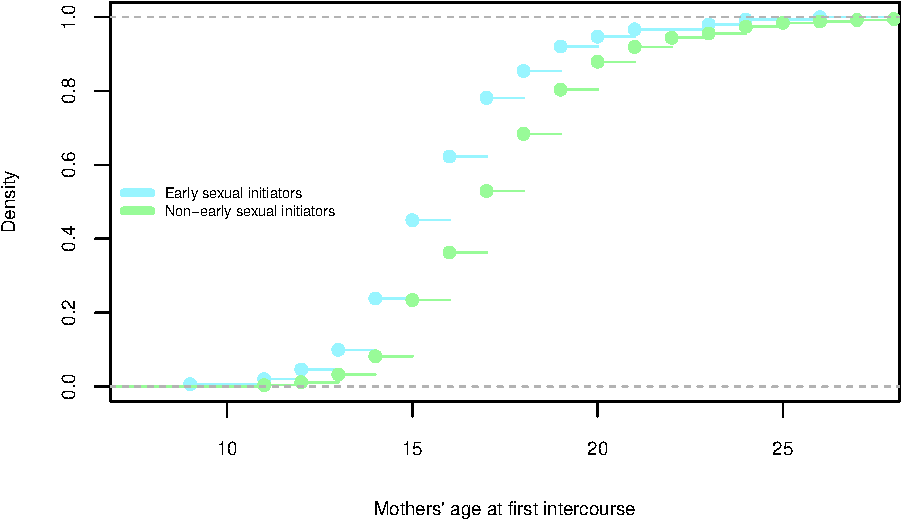
\includegraphics[width=0.8\linewidth,height=0.7\textheight]{early_sexual_activity_report_files/figure-latex/unnamed-chunk-4-1} 

}

\caption{Cumulative histogram of age at first intercourse of mothers by group}\label{fig:unnamed-chunk-4}
\end{figure}

Logistic regressions were used to assess the relationship between the
early onset of sexual activity among girls and the mothers' sexual
bargaining ability, as well as other behavioral traits such as the
mothers' age at first intercourse and whether she had a teenage birth.
Table 2 shows the coefficients (log odds ratio) of these regressions. To
observe the predicting ability of the three mother-related variables
(sexual bargaining, teenage birth, and age at first intercourse) alone
and in interaction, we computed three logistic regressions. Thus, we can
notice how the significance of the coefficient changes with each
additional variable. Each regression is represented by a separate column
in Table 2.

As demonstrated in column 2 of Table 2, after adjustment for all
covariates, having a mother who lacks sexual bargaining and a mother who
had a teenage birth significantly increases the log odds of early sexual
onset. These results support the hypothesis that the sexual attitudes
and behavior may be in some mechanism inherited from mother to daughter.
Similarly, column 3 of Table 2 shows that for each additional year that
the mother delays her sexual debut, the log odds of her daughter being
sexually active decrease. When the age at first intercourse of the
mother is added to the model, however, lacking sexual bargaining and
having a teenage birth become statistically insignificant due to the
correlation of predictors. A plausible explanation is that the age at
first intercourse explains whether the mother is sexually empowered and
whether she was once a teenage mother.

Although not the main focus of the study, it is worth examining whether
sexuality knowledge has a predictive value in the model. As shown in
Table 2, while knowledge about period, pregnancy, and AIDs are not
statistically significant in any of the regressions, from whom girls
acquire information about sexual relations seems to matter. Even after
controlling for school attendance and other covariates, girls who learn
about sex from family have higher odds of engaging in early sexual
activity than those who learn from school. It is also worth noting that
the sociodemographic variables do not appear to explain the differences
in early sexual onset. In contrast, missing school and having an
employed mother significantly increases the logs odds of early sexual
debut.

As mentioned before, data about smoking and drinking were not gathered
for all subjects in our sample. Therefore, a series of logistic
regressions were performed on a smaller sample in order to add the two
cofounders to the original model. These regressions are illustrated in
Table 3. However, it is important to emphasize that the probability of
falling into type 2 error increases as the sample becomes smaller. Thus,
while having more cofounders improves the accuracy of the outcomes,
reducing the sample size may as well affect the precision of the
estimates.

As expected, smoking and drinking were high predictors for precocious
sexual initiation. Table 3 shows that even after controlling for these
two additional variables, the log odds of early sexual onset decrease
for each additional year that the mother delays her sexual debut.
Interestingly, when adding these cofounders, from whom girls learn about
sexual relations and having an employed mother are no longer
significant. As with the previous regressions, attending school and
having a mother who finished primary school are associated with delayed
sexual activity.

\begin{table}[!htbp] \centering    \caption{Logistic Regression Results}    \label{}  \begin{tabular}{@{\extracolsep{5pt}}lD{.}{.}{-3} D{.}{.}{-3} D{.}{.}{-3} }  \\[-1.8ex]\hline  \hline \\[-1.8ex]   & \multicolumn{3}{c}{\textit{Dependent variable:}} \\  \cline{2-4}  \\[-1.8ex] & \multicolumn{1}{c}{Early sexual initiation} & \multicolumn{1}{c}{Teenage pregnancy} & \multicolumn{1}{c}{Contraception use} \\  \\[-1.8ex] & \multicolumn{1}{c}{(1)} & \multicolumn{1}{c}{(2)} & \multicolumn{1}{c}{(3)}\\  \hline \\[-1.8ex]   Mother lacks sexual empowerment & 0.495^{*} & 0.354 & 0.089 \\    & (0.288) & (0.410) & (0.607) \\    Mother had a teenage birth & 0.760^{***} & 0.697^{**} & -0.659 \\   &  &  &  \\   &  &  &  \\    & (0.198) & (0.288) & (0.421) \\    Mother has a job & 0.491^{**} & 0.377 & -0.358 \\    & (0.203) & (0.287) & (0.422) \\    Mother finished primary school & -0.801^{*} & -0.901 & 2.128^{*} \\    & (0.460) & (0.590) & (1.217) \\    Mother finished high school & -0.501 & -0.975 & 2.090^{*} \\    & (0.476) & (0.619) & (1.221) \\    Mother finished college & -0.563 & -0.703 & 3.666^{**} \\   &  &  &  \\  &  &  &  \\    & (0.546) & (0.736) & (1.468) \\    Misses school & 2.155^{***} & 2.157^{***} & -0.763 \\    & (0.285) & (0.324) & (0.468) \\    Lacked knowledge about period & 0.356 & 0.490 & -0.341 \\    & (0.222) & (0.305) & (0.450) \\    Knows about sexuality from family & 1.647^{***} & 1.474^{*} & 0.765 \\    & (0.574) & (0.791) & (1.324) \\    Knows about sexuality from school & 1.320^{**} & 1.266^{*} & -0.451 \\    & (0.514) & (0.706) & (1.239) \\    Knows about sexuality from other sources & 1.942^{***} & 1.541^{*} & 0.155 \\    & (0.661) & (0.895) & (1.400) \\   \hline \\[-1.8ex]  Household-related controls? & Yes & Yes & Yes \\  Observations & \multicolumn{1}{c}{981} & \multicolumn{1}{c}{981} & \multicolumn{1}{c}{159} \\  \hline  \hline \\[-1.8ex]  \textit{Note:}  & \multicolumn{3}{r}{$^{*}$p$<$0.1; $^{**}$p$<$0.05; $^{***}$p$<$0.01} \\  \end{tabular}  \end{table}

\hypertarget{discussion}{%
\subsection{DISCUSSION}\label{discussion}}

This study contributes to the literature on early initiation of sexual
activity among female adolescents. It is not the time maternal
empowerment has been studied as a predictor of sexual activity. Gipson
and Upchurch (2017), for instance, found that some of characteristics
and measures of maternal empowerment and status were predictive of their
daughters' sexual initiation. Yet, few if any have explored maternal
empowerment in the way it has been done in this study. In this research,
we found that girls who had a mother that was unable to turn down sex or
demand the use of contraception were more likely to be sexually active.
This raises the question of whether women's sexual behavior or
empowerment can be transmitted intergenerationally. It is worth noting
that sexual coercion is still a major cause of sexual debut (Moore et
al., 2007). In our sample, 34\% of girls reported not having agreed or
being convinced to engage in sexual activity at the time of their first
sexual experience. Perhaps, young women are able to mimic the sexual
conduct of their mothers. If submissive behavior is normalized within
the family, girls may find it acceptable to receive and accept sexual
advances against their will.

Another important outcome of this research was the relationship between
the timing of sexual onset among mothers and daughters. Even after
controlling for several cofounders, the mother's age at sexual debut was
one of the most significant and independent predictors. The younger a
mother was when she had her first intercourse, the higher the odds of
her daughter being sexually active by the age of 16. This finding is
parallel to the intergenerational tendency of early childbearing (Kahn
and Anderson, 1992), in which teenage mothers are more likely to have
been brought up by a single mother who had herself become a parent early
in her life. Previous research on sexual initiation has found that
adding drug use as a covariate largely impacts the significance of
coefficients (e.g.~Mandara et al., 2003). However, when smoking and
drinking were added into our models, the mother's age at first
intercourse remained statistically significant.

It is also worth discussing the interaction between sexual bargaining
and sexual onset among mothers. The mothers' sexual bargaining was a
good predictor of their daughters' sexual activity in the first models.
Nevertheless, when combined with the mothers' age at first coitus,
sexual bargaining was no longer significant, implying that sexual
bargaining predicted sexual activity through age at first coitus. These
findings strengthen the hypothesis of maternal empowerment as a
potential determinant of the timing of sexual debut. How much control
mothers have of their own sexual decision making may be mirrored in
their daughters' behavior. Mothers who started their sexual life
prematurely may have done so for reasons not necessarily attached to
their choice. These assumptions, however, need to be corroborated with
future research.

We found that girls whose mothers had completed primary school were less
likely to have engaged in sexual intercourse. These results are
consistent with previous evidence that has shown that maternal education
inhibits the risk of early sexual debut (e.g.~Brewster, 1994; Jordahl
and Lohman, 2009; Santelli et al., 2000). One explanation that has been
proposed is that better-educated parents have higher expectations for
their children to finish school and establish a career, putting pressure
on them to delay sexual onset (Guo et al., 2012). We also found that the
source from which girls received information about sexuality was a good
predictor of their sexual behavior. After controlling for school
attendance, girls who learned about sexuality from family were more
likely to have experienced sexual activity than their peers who reported
having learned from school. In Ecuador, parents have shown interest in
addressing sexuality with their children in order to discourage them
from having sexual relations. Yet, they face a few constraints,
including lack of knowledge and feelings of shame and anxiety (Jerves et
al., 2014). These limitations may hinder these efforts and even produce
unintended results. This may be one of the explanations why
communication from parent to child about sex was predictive of early
sexual activity.

To control for socioeconomic status, we also included measures such as
household income, access to internet, and household members. For
better-off households, we suspected that having a higher economic level
would likely increase the opportunity of having sexual relations
(e.g.~pregnancy). Yet, none of these variables was strongly predictive
of sexual debut. As for the mothers' employment, while we thought that
having a job would reduce the odds of precocious sexual initiation, we
found the opposite. Since the purpose of the survey was to gather data
about health and nutrition, it did not collect information about
parental monitoring. However, employed mothers may spend less time
supervising or parenting their daughters. Research findings are most
consistent that mother-child closeness and values towards sexual
relations are associated with lower risk of sexual activity (Sieving et
al., 2000).

Studies have shown that smoking and substance use among adolescents are
associated with early sexual activity (Bachanas et al., 2002; Mandara et
al., 2003; Robinson et al., 1999). In this study, we conducted a series
of separate models in which we included smoking and drinking as
cofounders. We had to reduce the sample size as data about these
specific risk factors were only obtained for a smaller group of
subjects. Yet, after adding these variables, the computed estimates were
large and significant. These findings corroborate previous research
showing that substance use plays a critical role in adolescents' sexual
decisions. Bachanas et al.~(2002) explored the predictive ability of
peer norms and substance use. They found that while both variables were
significantly associated with risky sexual behavior, only substance use
accounted for the variance in sexual behavior when combined in the same
model. Similarly, when we added smoking and drinking to the regressions,
communication about sexuality became no longer significant. These
results suggest that communication about sexuality was predictive of
sexual activity through substance use. Perhaps, parents who identify
deviant behavior in their children also include conversation about sex
when dealing with misconduct.

\hypertarget{conclusion}{%
\subsection{CONCLUSION}\label{conclusion}}

In this article, we discussed how maternal sexual empowerment was
related to female adolescents' sexual behavior. After controlling for
several confounders, we found that having a mother unable to turn down
sex or demand contraception increased the odds of early sexual
initiation. We also found that when adding mothers' age at first
intercourse, sexual empowerment was no longer significant. This suggests
that maternal sexual empowerment was predictive of sexual onset through
mothers' age at first intercourse. Perhaps, mothers who reported low
sexual empowerment did not have control of their sexual decisions at the
time of their first sexual encounter. We believe that in some manner,
these attitudes and values can be transmitted from mother to daughter.

Although the nature of this research does not allow for a causal
relationship to be established, we believe that female adolescents'
attitudes toward sex and the ability to refuse sexual intercourse may be
shaped somehow through their mothers' bargaining power in sexual
relationships. The traditional parental interventions designed to delay
sexual onset and promote contraception use focuses on improving
communication about sexuality. Yet, the results presented indicate that
interventions towards mothers' sexual empowerment may help girls,
especially at a very young age, to develop skills for managing sexual
relationships. New mechanisms in which maternal empowerment influences
daughters' outcomes yet need to be researched.

\hypertarget{references}{%
\subsection*{References}\label{references}}
\addcontentsline{toc}{subsection}{References}

\hypertarget{refs}{}
\begin{cslreferences}
\leavevmode\hypertarget{ref-bachanas2002predictors}{}%
Bachanas, P.J., Morris, M.K., Lewis-Gess, J.K., Sarett-Cuasay, E.J.,
Sirl, K., Ries, J.K., Sawyer, M.K., 2002. Predictors of risky sexual
behavior in african american adolescent girls: Implications for
prevention interventions. Journal of pediatric psychology 27, 519--530.

\leavevmode\hypertarget{ref-bellis2006adults}{}%
Bellis, M.A., Downing, J., Ashton, J., 2006. Adults at 12? Trends in
puberty and their public health consequences.

\leavevmode\hypertarget{ref-brewster1994race}{}%
Brewster, K.L., 1994. Race differences in sexual activity among
adolescent women: The role of neighborhood characteristics. American
Sociological Review 408--424.

\leavevmode\hypertarget{ref-ellis2003does}{}%
Ellis, B.J., Bates, J.E., Dodge, K.A., Fergusson, D.M., John Horwood,
L., Pettit, G.S., Woodward, L., 2003. Does father absence place
daughters at special risk for early sexual activity and teenage
pregnancy? Child development 74, 801--821.

\leavevmode\hypertarget{ref-finer2013sexual}{}%
Finer, L.B., Philbin, J.M., 2013. Sexual initiation, contraceptive use,
and pregnancy among young adolescents. Pediatrics 131, 886--891.

\leavevmode\hypertarget{ref-gipson2017status}{}%
Gipson, J.D., Upchurch, D.M., 2017. Do the status and empowerment of
mothers predict their daughters' reproductive outcomes? BMC pregnancy
and childbirth 17, 348.

\leavevmode\hypertarget{ref-guo2012timing}{}%
Guo, W., Wu, Z., Qiu, Y., Chen, G., Zheng, X., 2012. The timing of
sexual debut among chinese youth. International perspectives on sexual
and reproductive health 196--204.

\leavevmode\hypertarget{ref-inec2019}{}%
INEC, 2019. Encuesta de salud y nutricion 2018.

\leavevmode\hypertarget{ref-jerves2014understanding}{}%
Jerves, E., Lopez, S., Castro, C., Ortiz, W., Palacios, M., Rober, P.,
Enzlin, P., 2014. Understanding parental views of adolescent sexuality
and sex education in ecuador: A qualitative study. Sex Education 14,
14--27.

\leavevmode\hypertarget{ref-johnson2007adolescent}{}%
Johnson, K.A., Tyler, K.A., 2007. Adolescent sexual onset: An
intergenerational analysis. Journal of Youth and Adolescence 36,
939--949.

\leavevmode\hypertarget{ref-jordahl2009bioecological}{}%
Jordahl, T., Lohman, B.J., 2009. A bioecological analysis of risk and
protective factors associated with early sexual intercourse of young
adolescents. Children and Youth Services Review 31, 1272--1282.

\leavevmode\hypertarget{ref-kaestle2005young}{}%
Kaestle, C.E., Halpern, C.T., Miller, W.C., Ford, C.A., 2005. Young age
at first sexual intercourse and sexually transmitted infections in
adolescents and young adults. American journal of epidemiology 161,
774--780.

\leavevmode\hypertarget{ref-kahn1992intergenerational}{}%
Kahn, J.R., Anderson, K.E., 1992. Intergenerational patterns of teenage
fertility. Demography 29, 39--57.

\leavevmode\hypertarget{ref-magnusson2012early}{}%
Magnusson, B.M., Masho, S.W., Lapane, K.L., 2012. Early age at first
intercourse and subsequent gaps in contraceptive use. Journal of Women's
Health 21, 73--79.

\leavevmode\hypertarget{ref-mandara2003predictors}{}%
Mandara, J., Murray, C.B., Bangi, A.K., 2003. Predictors of african
american adolescent sexual activity: An ecological framework. Journal of
Black Psychology 29, 337--356.

\leavevmode\hypertarget{ref-meyer2003measuring}{}%
Meyer, B.D., Sullivan, J.X., 2003. Measuring the well-being of the poor
using income and consumption. National Bureau of Economic Research.

\leavevmode\hypertarget{ref-moore2007coerced}{}%
Moore, A.M., Awusabo-Asare, K., Madise, N., John-Langba, J.,
Kumi-Kyereme, A., 2007. Coerced first sex among adolescent girls in
sub-saharan africa: Prevalence and context. African journal of
reproductive health 11, 62.

\leavevmode\hypertarget{ref-newcomer1987parental}{}%
Newcomer, S., Udry, J.R., 1987. Parental marital status effects on
adolescent sexual behavior. Journal of Marriage and the Family 235--240.

\leavevmode\hypertarget{ref-o2001early}{}%
O'Donnell, L., O'Donnell, C.R., Stueve, A., 2001. Early sexual
initiation and subsequent sex-related risks among urban minority youth:
The reach for health study. Family planning perspectives 268--275.

\leavevmode\hypertarget{ref-parkes2011parenting}{}%
Parkes, A., Henderson, M., Wight, D., Nixon, C., 2011. Is parenting
associated with teenagers' early sexual risk-taking, autonomy and
relationship with sexual partners? Perspectives on sexual and
reproductive health 43, 30--40.

\leavevmode\hypertarget{ref-paul2000determinants}{}%
Paul, C., Fitzjohn, J., Herbison, P., Dickson, N., 2000. The
determinants of sexual intercourse before age 16. Journal of Adolescent
Health 27, 136--147.

\leavevmode\hypertarget{ref-robinson1999predictors}{}%
Robinson, K.L., Teiljohann, S.K., Price, J.H., 1999. Predictors of sixth
graders engaging in sexual intercourse. Journal of School Health 69,
369--375.

\leavevmode\hypertarget{ref-romer1999parental}{}%
Romer, D., Stanton, B., Galbraith, J., Feigelman, S., Black, M.M., Li,
X., 1999. Parental influence on adolescent sexual behavior in
high-poverty settings. Archives of pediatrics \& adolescent medicine
153, 1055--1062.

\leavevmode\hypertarget{ref-santelli2000association}{}%
Santelli, J.S., Lowry, R., Brener, N.D., Robin, L., 2000. The
association of sexual behaviors with socioeconomic status, family
structure, and race/ethnicity among us adolescents. American journal of
public health 90, 1582.

\leavevmode\hypertarget{ref-schreiner2015ecuador}{}%
Schreiner, M., 2015. Ecuador 2013 poverty probability index(PPI): Design
memo.

\leavevmode\hypertarget{ref-sieverding2005influence}{}%
Sieverding, J.A., Adler, N., Witt, S., Ellen, J., 2005. The influence of
parental monitoring on adolescent sexual initiation. Archives of
pediatrics \& adolescent medicine 159, 724--729.

\leavevmode\hypertarget{ref-sieving2000maternal}{}%
Sieving, R.E., McNeely, C.S., Blum, R.W., 2000. Maternal expectations,
mother-child connectedness, and adolescent sexual debut. Archives of
Pediatrics \& Adolescent Medicine 154, 809--816.

\leavevmode\hypertarget{ref-st1996examination}{}%
St Lawrence, J.S., Scott, C.P., 1996. Examination of the relationship
between african american adolescents' condom use at sexual onset and
later sexual behavior: Implications for condom distribution programs.
AIDS Education and Prevention.

\leavevmode\hypertarget{ref-stockl2013early}{}%
Stöckl, H., Kalra, N., Jacobi, J., Watts, C., 2013. Is early sexual
debut a risk factor for hiv infection among women in sub-saharan africa?
A systematic review. American Journal of Reproductive Immunology 69,
27--40.

\leavevmode\hypertarget{ref-velez2005family}{}%
Velez-Pastrana, M.C., Gonzadez-Rodriguez, R.A., Borges-Hernandez, A.,
2005. Family functioning and early onset of sexual intercourse in latino
adolescents. Adolescence 40.

\leavevmode\hypertarget{ref-knitr2015}{}%
Xie, Y., 2015. Dynamic documents with R and knitr, 2nd ed. Chapman;
Hall/CRC, Boca Raton, Florida.
\end{cslreferences}

\end{document}
